\chapter{Introducció}
\label{cap:int}

\section{Motivació}
Des de fa unes poques dècades, els ordinadors permeten emmagatzemar una àmplia varietat d'informació de manera fiable i replicada per a que puga sobreviure al pas del temps, mantenir-la organitzada per a que siga fàcilment utilitzable i fer-la accessible arreu del món i quasi universalment. Però durant segles, l'única forma de transmetre el coneixement i emmagatzemar-lo de manera més o menys segura ha sigut mitjançant l'escriptura. Precisament el fet de mantenir el coneixement en llibres, manuscrits primer i impresos després, que permeten la seva preservació i més fàcil difusió, ha sigut una de les principals bases de tot el desenvolupament del coneixement humà, especialment científic i tecnològic, arreu del món i és el principal motor pel qual avui gaudim d'unes millors condicions de vida que les dels nostres avantpassats.\\

Malauradament, els llibres manuscrits i impresos no sempre han tingut èxit en la seva missió de preservar el coneixement. Sols cal recordar el desastrós incendi de l'antiga Biblioteca d'Alexandria que provocà que milers d'obres d'autors de l'antiguitat es perderen per sempre. Ajudar a la preservació de la informació continguda en els llibres manuscrits i ajudar també a la cerca del contingut en aquests, són dos dels motius que van fer nàixer el reconeixement de text manuscrit (HTR, de l'anglès \emph{Handwriting Text Recognition}) a principis del segle XX.\\

Tot i el progrés aconseguit en els últims anys pel Reconeixement de Text Manuscrit, aquest encara té molts problemes per resoldre. Molts d'ells causats perquè la gran variabilitat que presenta el text, en quant a l'estil d'escriptura, no aporta cap informació rellevant per a la classificació dels símbols representats a les imatges i dificulta el seu reconeixement. Per exemple, un mateix autor no escriu un mateix símbol sempre de la mateixa forma, ni de la mateixa grandària i ni tan sols amb la mateixa orientació. Per això, un dels components fonamentals de qualsevol sistema de reconeixement de l'escriptura és la normalització d'aquest text a la imatge, un procés que tracta de reduir aquesta variabilitat.\\

Aquest projecte compara i quantifica les diferències entre dues alternatives per solucionar un dels problemes que forma part d'aquest procés de normalització: la segmentació del del cos central del text manuscrit. El cos central d'una línia de text manuscrit és aquella porció de la línia on resideix el cos central de cadascun dels símbols que formen el text. Les dues alternatives estudiades per a aquesta segmentació del cos central estan basades en un enfocament heurístic del problema, on un algorisme amb unes regles pre-establertes determina quina és la regió del cos central, i una altra basada en tècniques d'aprenentatge supervisat, on un humà ha segmentat manualment el cos central d'un conjunt d'imatges de mostra i ha entrenat el sistema per a que intente segmentar de manera semblant les noves imatges. Els detalls es veuran en el capítol \ref{cap:seg}.


\section{Reconeixement de formes}
El reconeixement de formes (de l'anglès \emph{Pattern Recognition}) és una branca de l'aprenentatge automàtic que té com a objectiu fer que una màquina (un ordinador) tinga la capacitat de discernir entre diferents objectes del seu entorn. El sistema pot percebre el seu entorn a partir de diferents sensors com poden ser càmeres fotogràfiques o de vídeo, micròfons, sensors làser, de temperatura, etc. L'objectiu és, a partir dels senyals obtinguts per aquests sensors, descobrir i atorgar un significat als diferents objectes representats en els senyals (típicament, assignar-los a una categoria) \cite{DH73}.\\

Existeixen dos grans grups de problemes de reconeixement de formes. El primer, com s'havia dit, consisteix en assignar una categoria a algun objecte representat per una imatge. Per exemple, donada una imatge que conté un símbol, decidir quin és aquest símbol d'entre un conjunt de possibilitats (reconèixer el símbol a la imatge). És diu d'aquests problemes que tenen un aprenentatge supervisat perquè al sistema se l'entrena amb senyals d'entrada prèviament etiquetats, de manera que puga aprendre quines són les propietats del senyal que determinen la seva categoria.\\

En el segon grup, no és disposa de les categories assignades al senyal durant l'etapa d'entrenament. L'objectiu d'aquest grup és descobrir propietats en el senyal d'entrada. Per exemple, assignar una categoria automàtica a cadascun dels senyals d'entrada (\emph{clustering}) o trobar un model (típicament probabilístic) que permeta representar les dades d'entrenament. \\

Són moltes les aplicacions que poden ser interpretats com un problema de reconeixement de formes, és per això, i gràcies a l'avanç en la tecnologia informàtica, que l'interès en aquest camp a crescut notablement en les darreres dècades. Algunes de les aplicacions del reconeixement de formes són:
\begin{itemize}
\item Aplicacions sobre el llenguatge humà: Reconeixement automàtic de text, reconeixement automàtic de la parla, traducció automàtica, etc.
\item Aplicacions sobre imatges: Reconeixement facial, detecció i classificació d'objectes, etc.
\item Medicina: Detecció de tumors, classificació de cromosomes, etc.
\item Física: Detecció i classificació de cossos celestes, detecció de partícules subatòmiques, etc.
\end{itemize}

En el cas de l'aprenentatge supervisat, que és el més estès i el que s'utilitzarà en una de les tècniques descrites en aquest treball per a la segmentació del cos central (veure secció \ref{sec:seg_nn}), el procés de reconeixement es fa seguint el següent procediment (veure figura \ref{fig:rf}).

\begin{enumerate}
\item \textbf{Preprocessament}: Al senyal se li apliquen diferents transformacions que tenen com a objectiu eliminar la informació no rellevant per a la classificació.
\item \textbf{Extracció de característiques}: El resultat del preprocessament sol ser un senyal amb un alt nombre de dimensions i això dificulta l'estimació dels models per a la classificació. Per això, es tracta de reduir aquest nombre de dimensions extraient el que s'anomenen ``característiques'' del senyal (informació més rellevant per a representar-lo), que no són més que una representació del senyal en un espai menor de dimensions.
\item \textbf{Aprenentatge}: S'aprèn un model per a classificar el senyal amb la informació aportada per les característiques del senyal d'entrada i el coneixement a priori sobre les dades i la tasca (categoria del senyal, probabilitats de les categories, etc). Aquesta fase sols és utilitzada durant l'aprenentatge del model.
\item \textbf{Classificació}: Una vegada l'aprenentatge està complet, s'utilitzen les característiques del senyal i el model obtingut en el pas anterior per a predir la categoria d'una nova observació del senyal.
\end{enumerate}

\begin{figure}
\centering
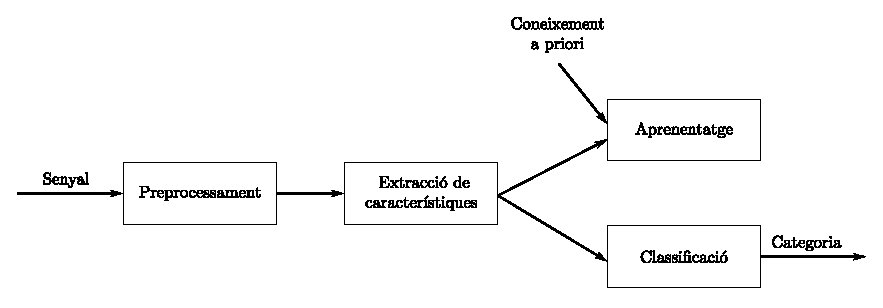
\includegraphics[width=\textwidth]{images/rf.eps}
\caption{Esquema d'un sistema de reconeixement de formes.}
\label{fig:rf}
\end{figure}

L'objectiu de l'aprenentatge supervisat pot interpretar-se com l'estimació d'una funció $g$ amb perfil $g : X \rightarrow C$, on $X$ és l'espai de característiques del senyal i $C$ el conjunt de categories; de manera que es minimitzen els errors de classificació per a un conjunt de dades d'entrenament $D = \{(x_1, c_1), (x_2, c_2), \ldots, (x_n, c_n)\}$ on $x_i$ és són les característiques obtingudes d'una mostra del senyal d'entrada i $c_i$ la seva categoria assignada. \\

La millor manera de construir aquesta funció és assignant la categoria $\hat{c}$ que maximitza la probabilitat de que les característiques del senyal observat representen aquesta categoria \cite{DH73}.
\begin{equation}\label{eq:bayes_classif}
g(x) = \argmax_{\forall c \in C} p(c|x) = \hat{c}
\end{equation}

L'equació \ref{eq:bayes_classif} pot escriure's de nou utilitzant el Teorema de Bayes segons l'equació \ref{eq:bayes_classif_v2} \cite{Bayes01011763}.

\begin{equation}\label{eq:bayes_classif_v2}
g(x) = \argmax_{\forall c \in C} \frac{p(c,x)}{p(x)} = \argmax_{\forall c \in C} \frac{p(x|c) p(c)}{p(x)} = \argmax_{\forall c \in C} p(x|c) p(c)
\end{equation}

Si es conegueren les distribucions exactes de $p(x|c)$ i $p(c)$, el problema de classificació quedaria resolt. Malauradament aquestes distribucions de probabilitat són desconegudes en les aplicacions reals i la major part del treball es concentra en trobar unes bones aproximacions d'aquestes a partir de les dades d'entrenament.

\section{Reconeixement de text manuscrit}
El reconeixement de text manuscrit (HTR, de l'anglès \emph{Handwriting Text Recognition}) començà a desenvolupar-se a principis del segle XX amb l'aparició de dispositius que permetien classificar dígits o caràcters manuscrits sobre sensors d'una determinada forma \cite{Goldberg1914}. A mitjans del segle XX aparegueren els primers dispositius que permetien introduir el resultat d'aquesta classificació en un ordinador \cite{10.1109/AFIPS.1957.60} i fins i tot sistemes que eren capaços de reconèixer paraules manuscrites aïllades \cite{Harmon1962}. Aquests primers dispositius estaven limitats per el desenvolupament tècnic d'aquell temps i solien necessitar-se dispositius especials sobre els que escriure el text. No era possible reconèixer el text d'un document manuscrit existent (com un llibre o un formulari). Fou més tard i gràcies a l'expansió de la informàtica quan els sistemes HTR començaren a adquirir la qualitat necessària per a aplicar-los en tasques de reconeixement real, com ara el reconeixement de dígits en xecs bancaris o el reconeixement de codis postals en el servei de correu.\\

Entre els sistemes HTR se'n diferencien dos tipus: el reconeixement \emph{online} i l'\emph{offline}. La diferència rau en el mètode en que el senyal d'entrada al sistema és adquirit. En els sistemes HTR \emph{online} el reconeixement es duu a terme en el mateix moment en el que s'escriu el text gràcies a l'ús de bolígrafs electrònics que capturen el moviment de l'eina d'escriptura, la velocitat d'escriptura, la pressió sobre la superfície, etc. El reconeixement \emph{offline} es duu a terme una vegada el text ja ha sigut escrit sobre una superfície (típicament paper). Un escànner, càmera fotogràfica o de vídeo obté llavors una imatge de la superfície que conté el text a reconèixer i aquest és el senyal a utilitzar pel sistema de reconeixement. Degut a que en el reconeixement \emph{online} es disposa d'informació temporal que no està disponible en el reconeixement \emph{offline}, es considera que el primer és un problema més senzill de resoldre (aconseguir sistemes amb un menor error de reconeixement).\\

Una altra divisió en les tasques de reconeixement de text, és si els símbols que apareixen es troben aïllats o són continus. En el reconeixement de símbols aïllats, cadascun dels símbols a reconèixer es troba ben separat de la resta (figura \ref{fig:text_segmentat}). No ocorre el mateix en el reconeixement de text continu, on pot haver diferents símbols units per un mateix traç (figura \ref{fig:text_continu}). En el sistema d'escriptura occidental, el text continu és el més habitual en el text manuscrit. El cas continu es considera més difícil ja que la forma d'un símbol depèn fortament dels seus adjacents i l'unió de certs símbols pot ocasionar ambigüitat i requereix més context (per exemple, ``rn'' o ``m'', ``vv'' o ``w'', etc).\\

\begin{figure}
\centering
\begin{subfigure}[b]{0.4\textwidth}
\centering
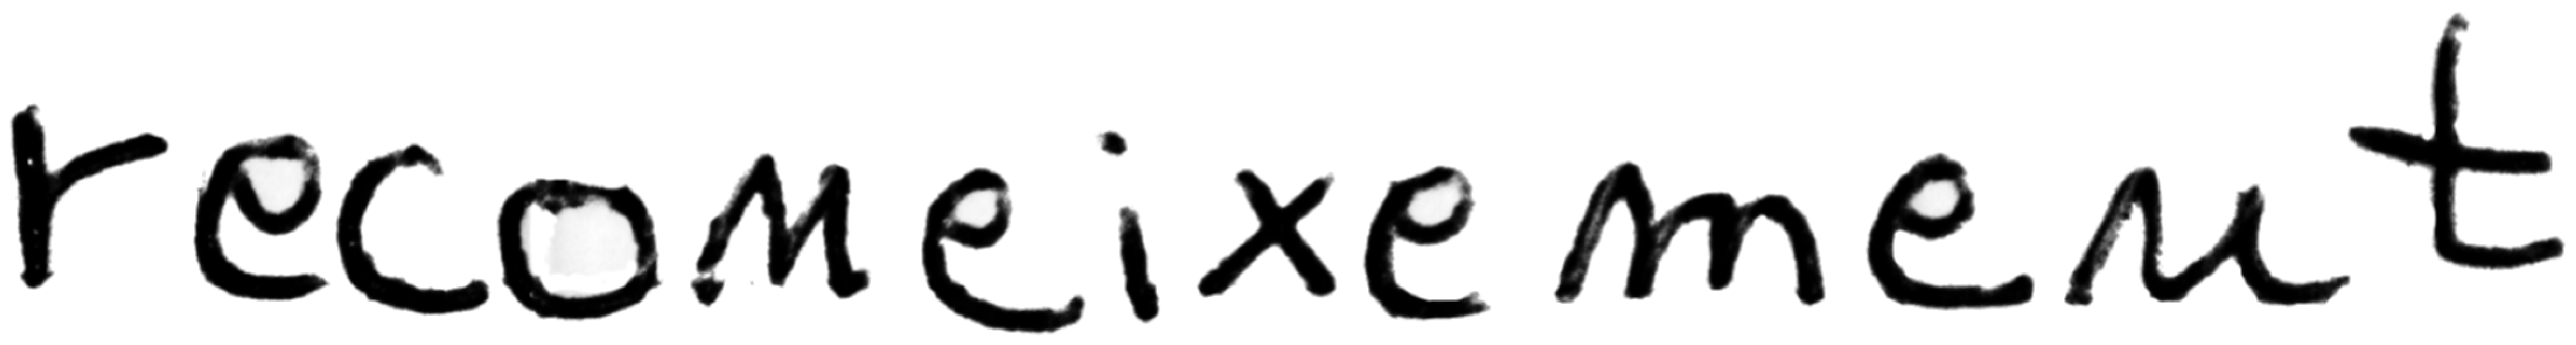
\includegraphics[width=\textwidth]{images/reconeixement_segmentat.eps}
\caption{Text amb símbols aïllats}\label{fig:text_segmentat}
\end{subfigure}
~
\begin{subfigure}[b]{0.4\textwidth}
\centering
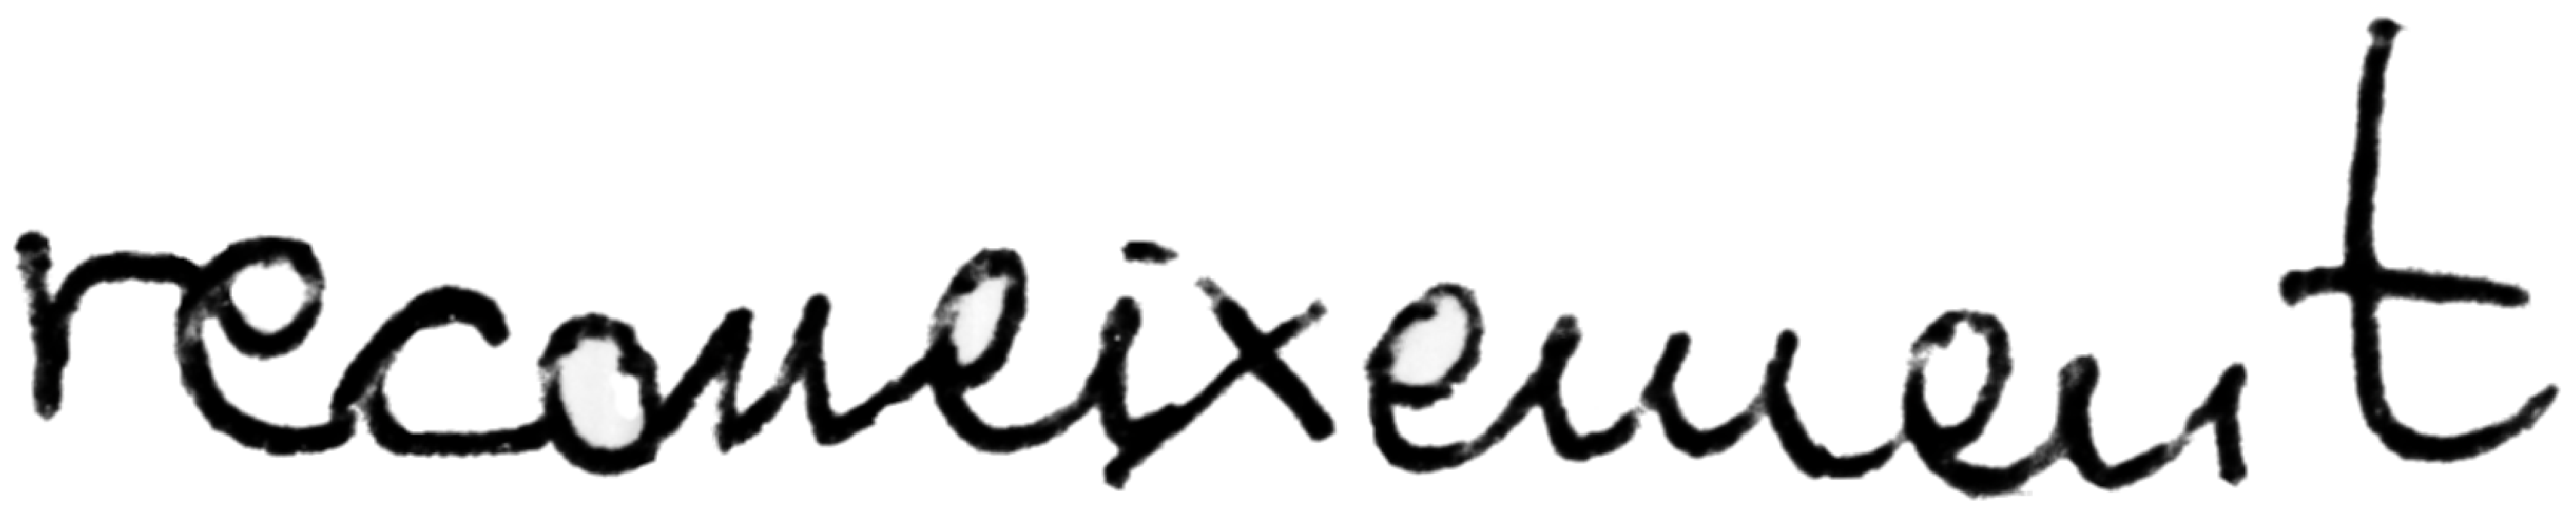
\includegraphics[width=\textwidth]{images/reconeixement_continu.eps}
\caption{Text amb símbols continu}\label{fig:text_continu}
\end{subfigure}
\caption{Dos exemples d'una paraula escrita amb text segmentat i continu.}
\end{figure}

Entre els principals problemes als que s'enfronta un bon sistema de reconeixement del text manuscrit són:
\begin{itemize}
\item \textbf{Soroll en les imatges}: la imatge capturada pot contenir soroll que depèn de l'eina d'escriptura (un bolígraf o un llapis), la superfície (paper o cartró) o el tipus d'eina d'adquisició i la seva qualitat.
\item \textbf{Diferents estils d'escriptura}: el mateix símbol és escrit de moltes formes, no sols depenent de l'autor, sinó també depenent del seu estat d'ànim, rapidesa en l'escriptura, context en el que es situa el símbol, etc.
\end{itemize}

L'etapa de preprocessament que es descrivia abans intenta per una banda eliminar o reduir el soroll en les imatges, i per altra, reduir les diferències en els estils d'escriptura. La correcta segmentació del cos central del text és important per aplicar certes transformacions que tenen com a objectiu la reducció d'aquest segon problema.\\

Aquest projecte s'ha realitzat en un context de reconeixement de text manuscrit \emph{offline} i continu, encara que els mètodes estudiats en aquest projecte per a la segmentació del cos central del text poden ser utilitzats igualment en un entorn de text segmentat.\\

Podem aplicar l'equació \ref{eq:bayes_classif} que s'havia presentat anteriorment per solucionar el problema del reconeixement de text \emph{offline}. Suposem que disposem d'una imatge $I$ que conté cert text, llavors l'objectiu és trobar la seqüència de símbols $\hat{s} = s_1, s_2, \ldots, s_N$ que maximitza la probabilitat de que aquests símbols siguen els representats a la imatge $I$.

\begin{equation}\label{eq:}
\hat{s} = \argmax_{s \in \Sigma^*} p(s|I)
\end{equation}

En el cas del reconeixement de text \emph{offline} i continu, típicament s'extreu una seqüència de vectors de característiques $\vec{x} = \vec{x}_1, \vec{x}_2, \ldots \vec{x}_T$ a partir de la imatge $I$. Aquests vectors s'extreuen a partir d'una finestra lliscant d'anàlisi que travessa tota la imatge. Per a cada posició on es fixa aquesta finestra, s'extreu un vector de característiques. La figura \ref{fig:finestra_lliscant} mostra aquesta finestra. Per tant, el reconeixement es reduiria a trobar la seqüència $\hat{s}$ que maximitza la probabilitat en  \ref{eq:bayes_classif}

\begin{equation}\label{eq:bayes_classif_vectors}
\hat{s} = \argmax_{s \in \Sigma^*} p(s|\vec{x}) = \argmax_{s \in \Sigma^*} p(\vec{x}|s) p(s) %= \argmax_{s \in \Sigma^*} p(\vec{x}_1, \vec{x}_2, \ldots \vec{x}_T | s) p(s)
\end{equation}

\begin{figure}
\centering
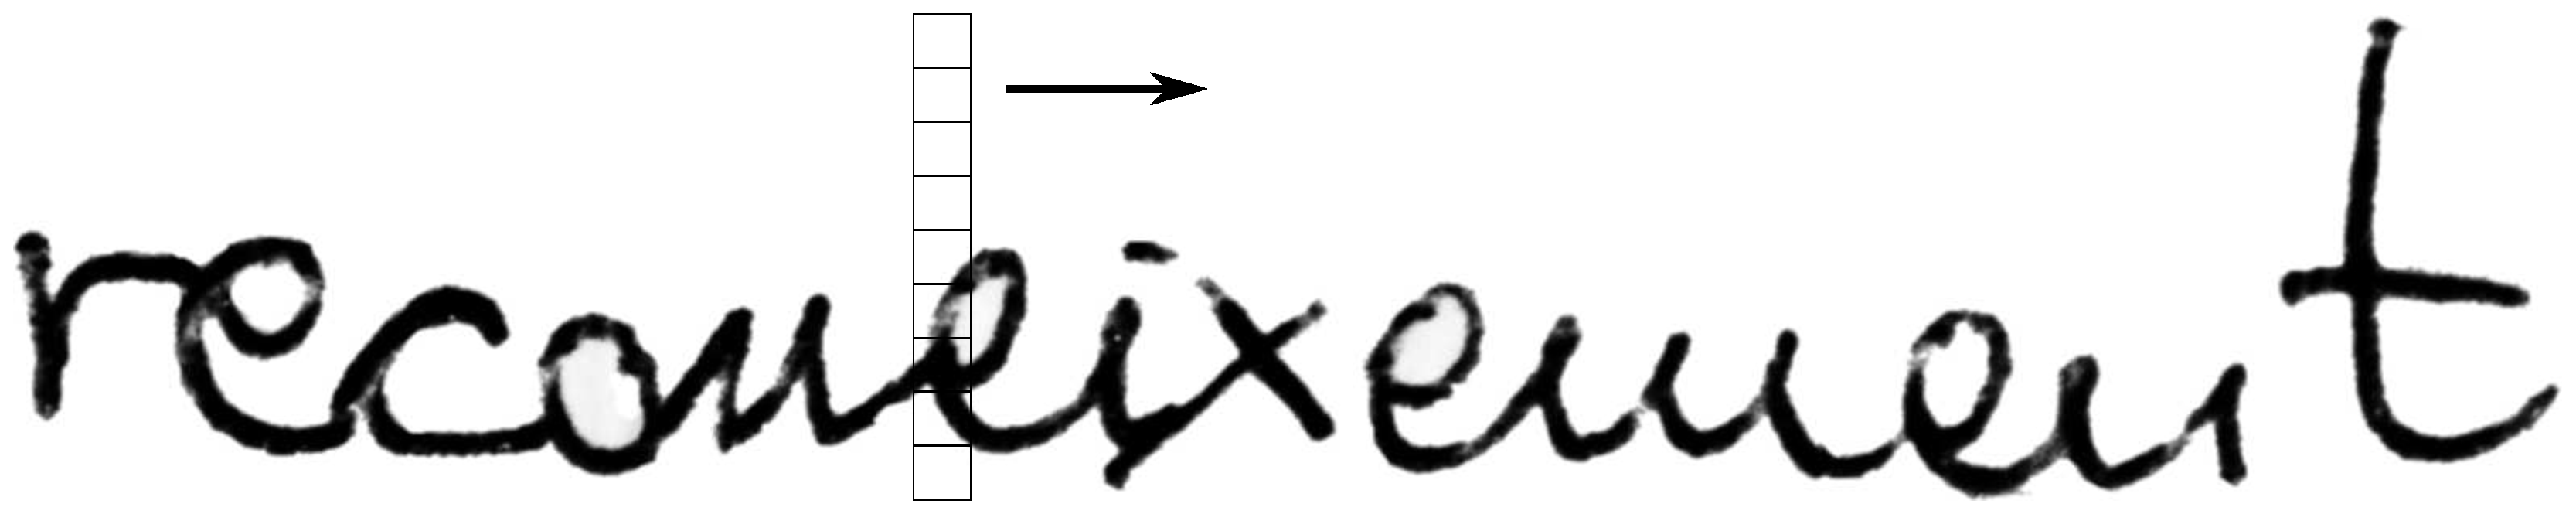
\includegraphics[width=0.8\textwidth]{images/finestra_lliscant.eps}
\caption{Finestra lliscant d'anàlisi en una imatge}
\label{fig:finestra_lliscant}
\end{figure}

Habitualment, tant en entorns de reconeixement de text com de veu, la distribució a posteriori $p(\vec{x}|s)$ es modela utilitzant Models Ocults de Markov (HMM, de l'anglès \emph{Hidden Markov Models}) i Models de Mixtures Gaussianes (GMM, de l'anglès \emph{Gaussian Mixture Models}) \cite{huanghidden, jelinek1998statistical, ghahramani2001introduction} i $p(s)$ es modela utilitzant models de llenguatge de $n$-grames \cite{jelinek1998statistical,katz1987estimation,marti2001using}. Aquesta és l'aproximació que s'ha utilitzat en aquest projecte.